% IEEE Conference Paper - 4 Pages, 2-Sided
% Physics-Informed Deep State Estimation Benchmark
\documentclass[conference]{IEEEtran}

% ---- Packages ----
\usepackage{cite}
\usepackage{amsmath,amssymb,amsfonts}
\usepackage{graphicx}
\usepackage{textcomp}
\usepackage{booktabs}
\usepackage{url}

\graphicspath{{figures/}}

\begin{document}

\title{Physics-Informed Deep State Estimation Under\\Sensor Dropout in Radial Distribution Networks:\\MLP, GNN, and TCN Trade-offs}

\author{
\IEEEauthorblockN{Vinayak Singh}
\IEEEauthorblockA{Department of Electrical Engineering\\
Institution Name\\
City, Country\\
email@institution.edu}
}

\maketitle

% ============================================================
% ABSTRACT
% ============================================================
\begin{abstract}
Data-driven Distribution System State Estimation (DSSE) promises real-time grid monitoring, yet most published models are evaluated under ideal telemetry conditions, masking severe failure modes under sensor dropout. This paper benchmarks three physics-informed deep learning architectures---a global dense Multi-Layer Perceptron (MLP), a topology-aware Edge-Attributed Graph Neural Network (GNN), and a causal Temporal Convolutional Network (TCN)---on the IEEE 33-bus feeder with 16~PMUs (${\sim}50\%$ coverage) under 10\%--50\% random sensor blackouts and ${\pm}10\%$ pseudo-measurement noise.

Three key trends emerge from the results. First, an \textit{accuracy--resilience trade-off}: under clean (unprepared) training, a 50\% PMU blackout causes the MLP error to spike by $+164\%$, while the TCN absorbs it with only $+25.7\%$ growth owing to its 12-hour temporal memory. With dropout-augmented training, the MLP reclaims top accuracy ($|V|$~RMSE~$=0.000515$~pu, $0.223$~ms latency). Second, a \textit{topological horizon}: the 3-layer GNN cannot propagate information across the 17-hop radial feeder, capping its accuracy at $0.001295$~pu. Third, a \textit{physics regularization Pareto cliff}: moderate AC power-flow penalties ($\lambda \in [0.001, 0.1]$) improve estimation, but aggressive weights ($\lambda \ge 10.0$) degrade performance by forcing models to fit noisy pseudo-measurements. These findings provide practical guidelines for selecting DSSE architectures under real-world telemetry failures.
\end{abstract}

\begin{IEEEkeywords}
Distribution system state estimation, physics-informed neural network, graph neural network, temporal convolutional network, PMU dropout, IEEE 33-bus
\end{IEEEkeywords}

% ============================================================
% I. INTRODUCTION
% ============================================================
\section{Introduction}

Distribution System State Estimation (DSSE) reconstructs the voltage magnitude and phase angle at every bus from incomplete sensor readings. The conventional approach uses Weighted Least Squares (WLS) optimization \cite{schweppe1970}, which iteratively solves:
\begin{equation}
    \hat{\mathbf{x}} = \arg\min_{\mathbf{x}} \left[\mathbf{z} - \mathbf{h}(\mathbf{x})\right]^T \mathbf{R}^{-1} \left[\mathbf{z} - \mathbf{h}(\mathbf{x})\right]
    \label{eq:wls}
\end{equation}
where $\mathbf{z}$ is the measurement vector, $\mathbf{h}(\cdot)$ is the nonlinear measurement function, and $\mathbf{R}$ is the noise covariance matrix. While WLS is well established for transmission grids, it faces challenges in distribution networks: low redundancy from sparse Phasor Measurement Unit (PMU) deployments causes unobservability, and communication dropouts during extreme events cause the iterative solver to diverge \cite{primadianto2017}.

Deep learning offers a non-iterative alternative, mapping measurements directly to state estimates in a single forward pass. However, prior data-driven approaches suffer from key limitations. Standard black-box models ignore physical laws and degrade catastrophically under sensor dropout \cite{mestav2019}. Current-injection Physics-Informed Neural Networks (PINNs) assume known power injections at all buses \cite{iliadis2025}. TCN autoencoders relying on constant-Jacobian decoders require observable pre-training \cite{raghuvamsi2024}. Hybrid GNN-Kalman methods need localized full-PMU zones \cite{ngo2024}, and physics-embedded Graph Attention Networks involve multi-stage SCADA-dependent pipelines designed for transmission grids \cite{hu2025}.

This paper makes the following contributions:
\begin{enumerate}
    \item A unified benchmark comparing three deep learning paradigms---global spatial (MLP), topological (GNN), and temporal (TCN)---under identical conditions on a radial distribution feeder.
    \item An explicit evaluation of \textit{clean-trained} versus \textit{augmented-trained} models under up to 50\% sensor blackout, quantifying the accuracy--resilience trade-off.
    \item Identification of two practical design limits: the \textit{topological horizon} of message-passing GNNs on long radial feeders, and the \textit{Pareto cliff} of physics regularization under noisy pseudo-measurements.
\end{enumerate}

% ============================================================
% II. RELATED WORK
% ============================================================
\section{Related Work}

Table~\ref{tab:literature} summarizes the positioning of this work against six baseline methodologies. Classical WLS \cite{schweppe1970} diverges under unobservability. Black-box deep learning models map $\mathbf{z} \to \mathbf{x}$ effectively but violate power-flow physics and exhibit catastrophic out-of-distribution (OOD) failure under sensor dropout. Iliadis~et~al.~\cite{iliadis2025} embed current-injection physics into the loss, but assume known injections at all buses. Raghuvamsi~\cite{raghuvamsi2024} proposes a TCN autoencoder with a constant-Jacobian decoder, requiring full-observability pre-training. Ngo~et~al.~\cite{ngo2024} fuse a GNN with local Kalman filters but need dedicated full-PMU zones. Hu~et~al.~\cite{hu2025} deploy a physics-embedded GAT in a multi-stage SCADA pipeline designed for transmission grids.

In contrast, our study evaluates three single-stage architectures on a \textit{distribution} feeder under realistic partial observability and progressive sensor dropout, without requiring SCADA baselines, full-PMU zones, or constant-Jacobian assumptions.

\begin{table}[t]
\centering
\caption{Positioning Against Prior DSSE Methods}
\label{tab:literature}
\footnotesize
\setlength{\tabcolsep}{3pt}
\begin{tabular}{p{1.8cm}p{2.2cm}p{3.5cm}}
\toprule
\textbf{Method} & \textbf{Mechanism} & \textbf{Limitation Addressed by This Work} \\
\midrule
WLS \cite{schweppe1970} & Gauss-Newton & Diverges under dropout; our models are non-iterative ($0.22$--$2.20$~ms) \\
\addlinespace
Black-box DL & Supervised $\mathbf{z}{\to}\mathbf{x}$ & OOD collapse ($+164\%$); we quantify and resolve via augmentation/TCN \\
\addlinespace
PINN \cite{iliadis2025} & Current-injection loss & Assumes exact injections; we handle ${\pm}10\%$ noise and identify the Pareto cliff \\
\addlinespace
TCN Autoenc. \cite{raghuvamsi2024} & Constant-Jacobian decoder & Needs observable pre-training; our TCN learns nonlinear AC mappings directly \\
\addlinespace
GNN-Kalman \cite{ngo2024} & Zonal Kalman + GNN & Needs full-PMU zones; we expose the topological horizon with single-stage GNN \\
\addlinespace
GAT \cite{hu2025} & SCADA + GAT pipeline & Multi-stage, transmission-only; we benchmark on distribution feeder \\
\bottomrule
\end{tabular}
\end{table}

% ============================================================
% III. METHODOLOGY
% ============================================================
\section{Methodology}

\subsection{Problem Formulation}

The state vector $\mathbf{x} = [|\mathbf{V}|, \boldsymbol{\theta}]^T \in \mathbb{R}^{2N}$ contains the voltage magnitude and phase angle at each of the $N = 33$ buses. The measurement vector $\mathbf{z}$ combines PMU readings ($|V_i|$, $\theta_i$ at metered buses) with pseudo-measurements (forecast-based real and reactive power injections $P_i$, $Q_i$ at unmetered buses). The goal is to learn a mapping $f_\phi: \mathbf{z} \to \hat{\mathbf{x}}$ that minimizes prediction error while respecting AC power-flow physics.

\subsection{Model Architectures}

\textbf{Multi-Layer Perceptron (MLP).} A 4-layer fully connected network with 1024 hidden units per layer, ReLU activations, and batch normalization. The input is a 78-dimensional snapshot vector containing all available PMU and pseudo-measurement values. Because every input element connects to every neuron, the MLP can capture cross-correlations between all 33 buses in a single dense forward pass.

\textbf{Edge-Attributed Graph Convolutional Network (GNN).} A 3-layer Graph Convolutional Network with 128 hidden units per layer (86,402 parameters). Each edge is attributed with the physical line admittance features $[G_{ij}, B_{ij}, |Y_{ij}|, \angle Y_{ij}]$ derived from the bus admittance matrix $\mathbf{Y}_{\text{bus}}$. Message passing propagates information along the grid topology, so each layer extends the receptive field by one hop.

\textbf{Temporal Convolutional Network (TCN).} A causal 1D convolutional network with kernel size 3 and exponentially increasing dilations ($1, 2, 4, 8, 16$). This design gives a receptive field spanning approximately 12 hours of historical measurements. The causal structure ensures that only past observations influence the current estimate, preventing information leakage from the future.

\subsection{Physics-Informed Loss Function}

All three models are trained with a composite loss:
\begin{equation}
    \mathcal{L} = \mathcal{L}_{\text{MSE}} + \lambda \, \mathcal{L}_{\text{phys}}
    \label{eq:loss}
\end{equation}

The data term $\mathcal{L}_{\text{MSE}}$ penalizes the squared error between predicted and true bus states. The physics term enforces AC power-flow consistency by computing the apparent power residual:
\begin{equation}
    \mathbf{S}_{\text{calc}} = \hat{\mathbf{V}} \odot \left(\hat{\mathbf{V}} \, \mathbf{Y}_{\text{bus}}^T\right)^{*}
    \label{eq:physics}
\end{equation}

The residual between $\mathbf{S}_{\text{calc}}$ and the pseudo-measured injections $(P_{ps}, Q_{ps})$ forms $\mathcal{L}_{\text{phys}}$. Unlike \cite{iliadis2025}, which assumes exact current injections, we acknowledge that pseudo-measurements carry ${\pm}10\%$ forecast noise, making $\lambda$ a critical tuning parameter.

% ============================================================
% IV. EXPERIMENTAL SETUP
% ============================================================
\section{Experimental Setup}

\subsection{Test System}

We use the IEEE 33-bus radial distribution feeder \cite{baran1989}, which has 33 buses, 32 branches, and a topological diameter of 17 hops from the slack bus (bus~0, $|V|=1.0$~pu, $\theta=0.0$~rad) to the farthest leaf node. Sixteen PMUs are placed across non-slack buses, providing approximately 50\% direct observability.

\subsection{Noise Model}

PMU measurements are corrupted with Gaussian noise: $\sigma_{|V|} = 0.001$~pu and $\sigma_\theta = 0.05^\circ$. At unmetered buses, real and reactive power pseudo-measurements are generated from load forecasts with ${\pm}10\%$ Gaussian noise, reflecting practical forecast uncertainty in distribution networks.

\subsection{Training Regimes}

Two training protocols are used to study robustness:
\begin{itemize}
    \item \textbf{Clean Training:} All 16 PMUs are available during training. At test time, 10\%--50\% of PMUs are randomly dropped to simulate unexpected communication failures.
    \item \textbf{Augmented Training:} During each training epoch, 0\%--50\% of PMUs are randomly masked. This teaches the model to impute missing sensor readings.
\end{itemize}

Each architecture is trained across a sweep of physics weights $\lambda \in \{0, 10^{-4}, 10^{-3}, 10^{-2}, 10^{-1}, 1, 10, 100, 1000\}$ and evaluated at five dropout levels (10\%--50\%).

\begin{table}[t]
\centering
\caption{Architecture Specifications}
\label{tab:arch}
\footnotesize
\begin{tabular}{lccc}
\toprule
\textbf{Property} & \textbf{MLP} & \textbf{GNN} & \textbf{TCN} \\
\midrule
Input & 78-dim vector & Per-node features & 12-h time window \\
Hidden layers & 4 $\times$ 1024 & 3 $\times$ 128 & 5 dilated blocks \\
Parameters & ${\sim}3.2$M & 86,402 & ${\sim}150$K \\
Receptive field & All 33 buses & 3 hops & 12 hours \\
Best $\lambda$ (Aug.) & 0.1 & 0.001 & 0.01 \\
\bottomrule
\end{tabular}
\end{table}

% ============================================================
% V. RESULTS AND DISCUSSION
% ============================================================
\section{Results and Discussion}

\subsection{Trend 1: Accuracy--Resilience Trade-off}

The most striking trend in our results is the divergence between accuracy under controlled conditions and resilience under surprise failures. Fig.~\ref{fig:dropout} illustrates this clearly.

Under \textbf{clean training}, where models have never seen missing sensors, increasing the PMU dropout from 10\% to 50\% reveals dramatically different behaviors. The MLP's $|V|$ RMSE rises from $0.000772$~pu to $0.002038$~pu---a $+164\%$ increase. The GNN shows a similar upward trend, climbing from $0.001497$~pu to $0.002117$~pu ($+41.4\%$). By contrast, the TCN only rises from $0.001058$~pu to $0.001330$~pu ($+25.7\%$).

This trend has a clear explanation. The TCN maintains a 12-hour sliding window of past measurements. Because power system loads change gradually---a neighborhood's demand does not jump randomly from one instant to the next---the TCN can rely on recent historical context when current readings vanish. This temporal inertia acts as an implicit backup during sensor blackouts. The MLP, which sees only the present snapshot, has no such fallback; zeroed-out sensor values propagate directly into every neuron.

Under \textbf{augmented training}, the picture reverses. The MLP, now trained to expect missing sensors, becomes the accuracy champion: $|V|$ RMSE of $0.000515$~pu at 50\% dropout (Table~\ref{tab:results}). This is because the MLP's dense all-to-all connections allow it to learn cross-correlations between every pair of buses. When trained with random masking, it effectively learns to reconstruct any missing bus from the surviving ones.

\begin{figure}[t]
    \centering
    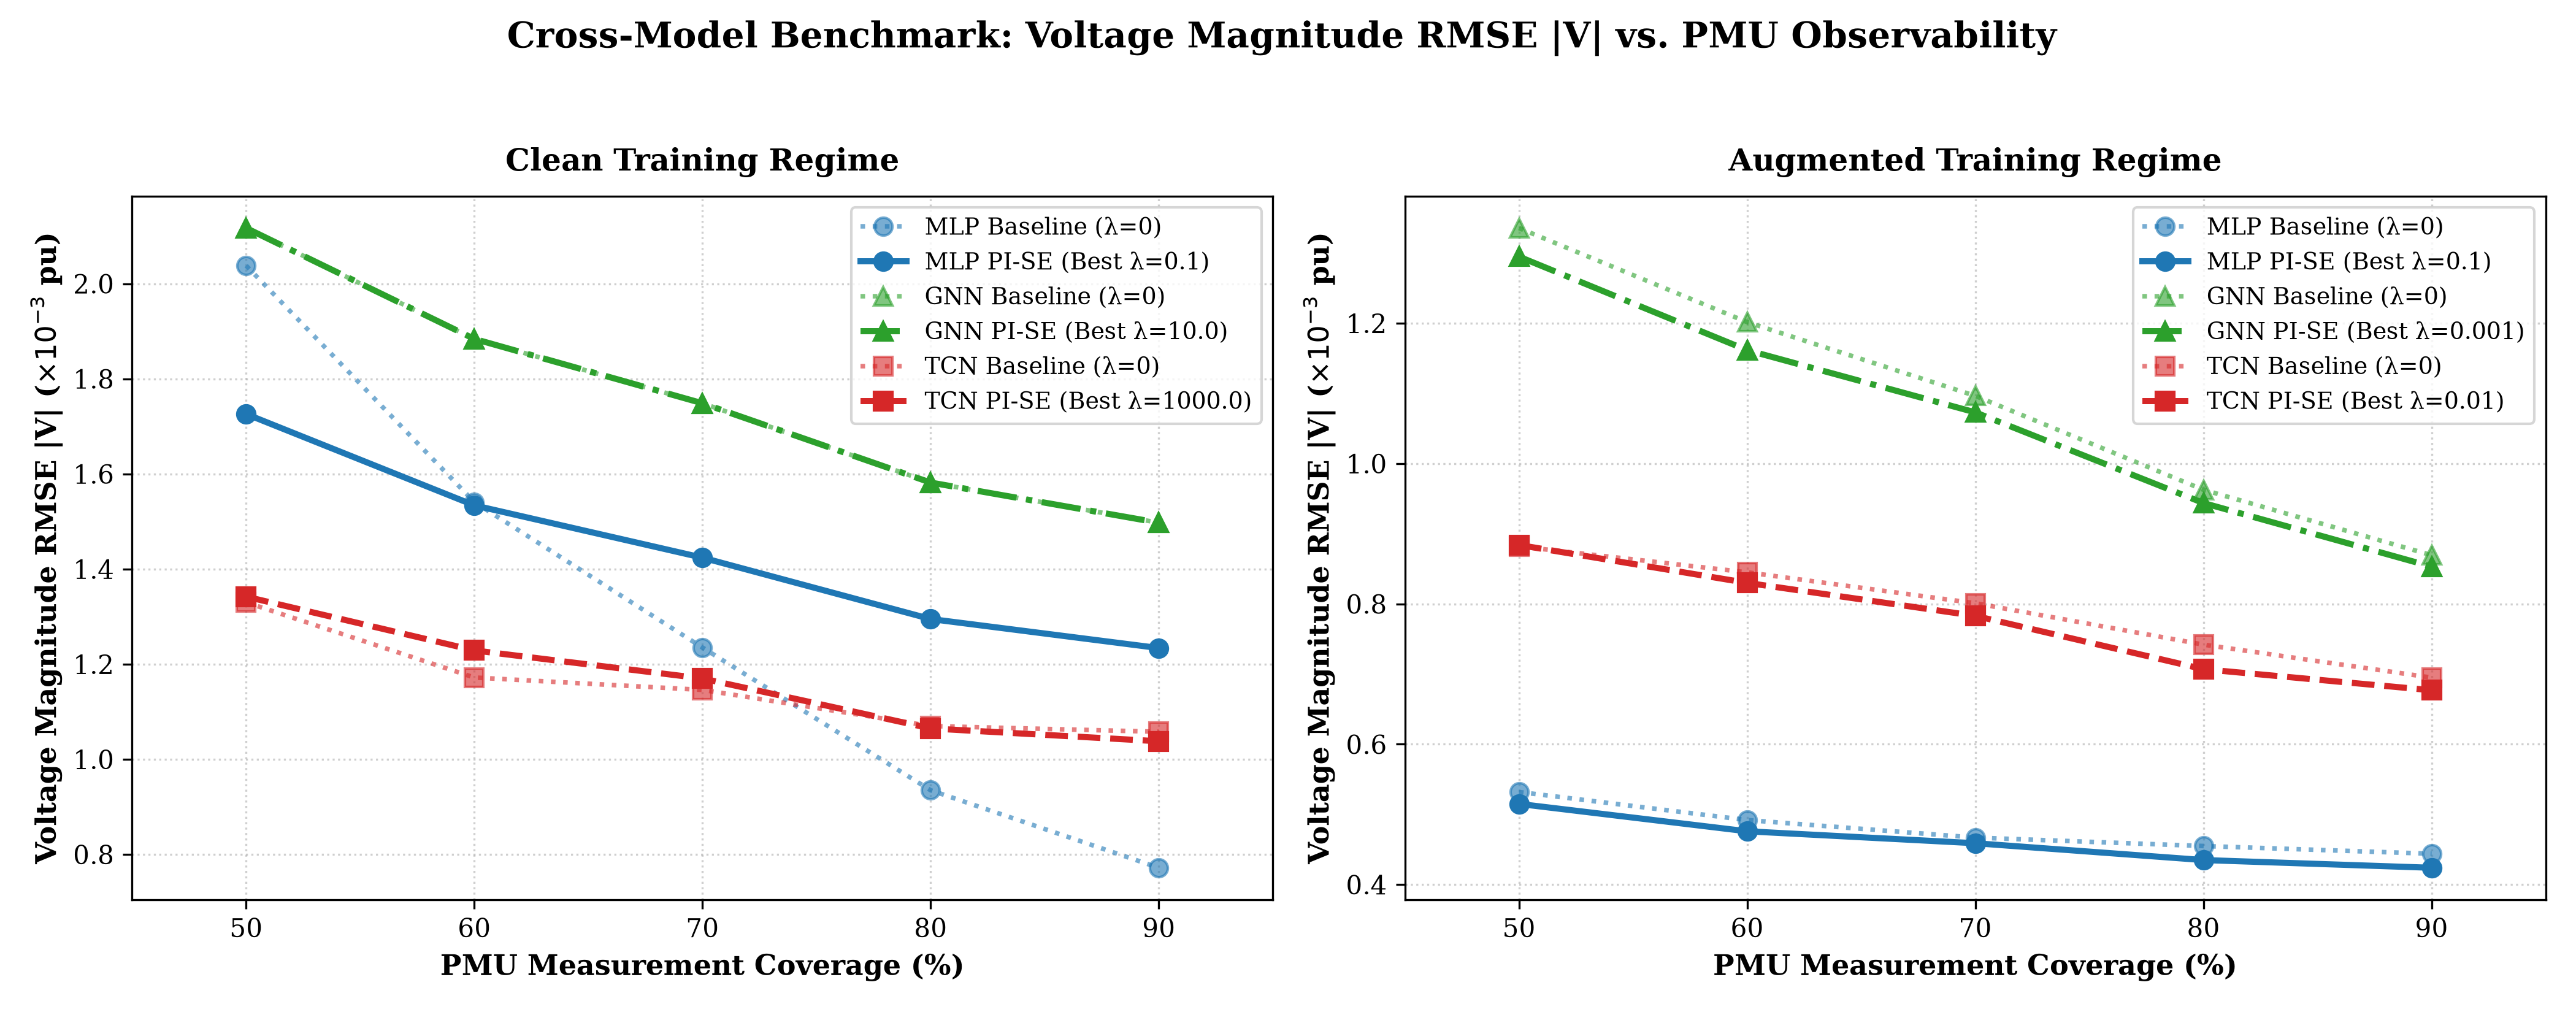
\includegraphics[width=\columnwidth]{vm_rmse_vs_coverage_comparison.png}
    \caption{Voltage magnitude RMSE versus PMU coverage for all three models under clean and augmented training. The MLP shows steep degradation under clean training while the TCN remains stable. With augmented training, all models improve, with the MLP achieving the lowest absolute error.}
    \label{fig:dropout}
\end{figure}

\begin{table}[t]
\centering
\caption{Performance at 50\% PMU Dropout (Best $\lambda$ per Model)}
\label{tab:results}
\footnotesize
\begin{tabular}{llccc}
\toprule
\textbf{Regime} & \textbf{Model} & \textbf{$|V|$ RMSE (pu)} & \textbf{$\theta$ RMSE ($^\circ$)} & \textbf{$\Delta$ from 10\%} \\
\midrule
Clean & MLP & $2.038 \times 10^{-3}$ & 0.0271 & $+164.0\%$ \\
Clean & GNN & $2.117 \times 10^{-3}$ & 0.0351 & $+41.4\%$ \\
Clean & TCN & $1.330 \times 10^{-3}$ & 0.0250 & $+25.7\%$ \\
\midrule
Augmented & MLP & $5.15 \times 10^{-4}$ & 0.0138 & $+21.5\%$ \\
Augmented & GNN & $1.295 \times 10^{-3}$ & 0.0223 & $+51.8\%$ \\
Augmented & TCN & $8.84 \times 10^{-4}$ & 0.0167 & $+30.6\%$ \\
\bottomrule
\end{tabular}
\end{table}

\subsection{Trend 2: The Topological Horizon of GNNs}

A consistent trend across both training regimes is that the GNN underperforms the MLP and TCN. Under augmented training at 50\% dropout, the GNN achieves $|V|$ RMSE of $0.001295$~pu---roughly $2.5\times$ worse than the MLP ($0.000515$~pu) and $1.5\times$ worse than the TCN ($0.000884$~pu).

This can be traced to a structural limitation we term the \textit{topological horizon}. In a graph neural network, each message-passing layer extends a node's receptive field by exactly one hop along the graph. With 3 layers, a node can aggregate information from at most 3 hops away. However, the IEEE 33-bus feeder is a long radial chain with a topological diameter of 17 hops. A bus at the far end of a lateral branch simply cannot receive any signal from a PMU located 12 or 15 hops away.

Stacking additional GNN layers is not a practical solution. Deep graph networks suffer from \textit{oversmoothing}, where node features converge to indistinguishable representations, and each additional layer adds latency. This horizon effect explains why prior GNN-based DSSE methods~\cite{ngo2024, hu2025} augmented their architectures with Kalman filters or SCADA baselines.

\subsection{Trend 3: The Physics Regularization Pareto Cliff}

Fig.~\ref{fig:lambda} shows the effect of varying the physics weight $\lambda$ on estimation accuracy. A clear trend emerges across all three models: moderate values of $\lambda$ ($0.001$ to $0.1$) either maintain or slightly improve accuracy over the unregularized baseline, while large values ($\lambda \ge 10.0$) cause a sharp degradation.

The root cause is the nature of the physics constraint. The AC power-flow residual (Eq.~\ref{eq:physics}) is computed against pseudo-measurements at unmetered buses, which carry ${\pm}10\%$ forecast noise. At moderate $\lambda$, the physics term acts as a soft guardrail---it steers predictions toward physically plausible voltage profiles without overpowering the data-driven loss. At high $\lambda$, the model is forced to satisfy power-flow equations that are themselves contaminated by forecast errors. The model effectively starts fitting the noise in the pseudo-measurements at the expense of matching true PMU readings.

This \textit{Pareto cliff} has a practical implication: physics-informed regularization is beneficial only when calibrated against the quality of available pseudo-measurements. For the best augmented models, the optimal $\lambda$ values were $0.1$ (MLP), $0.001$ (GNN), and $0.01$ (TCN).

\begin{figure}[t]
    \centering
    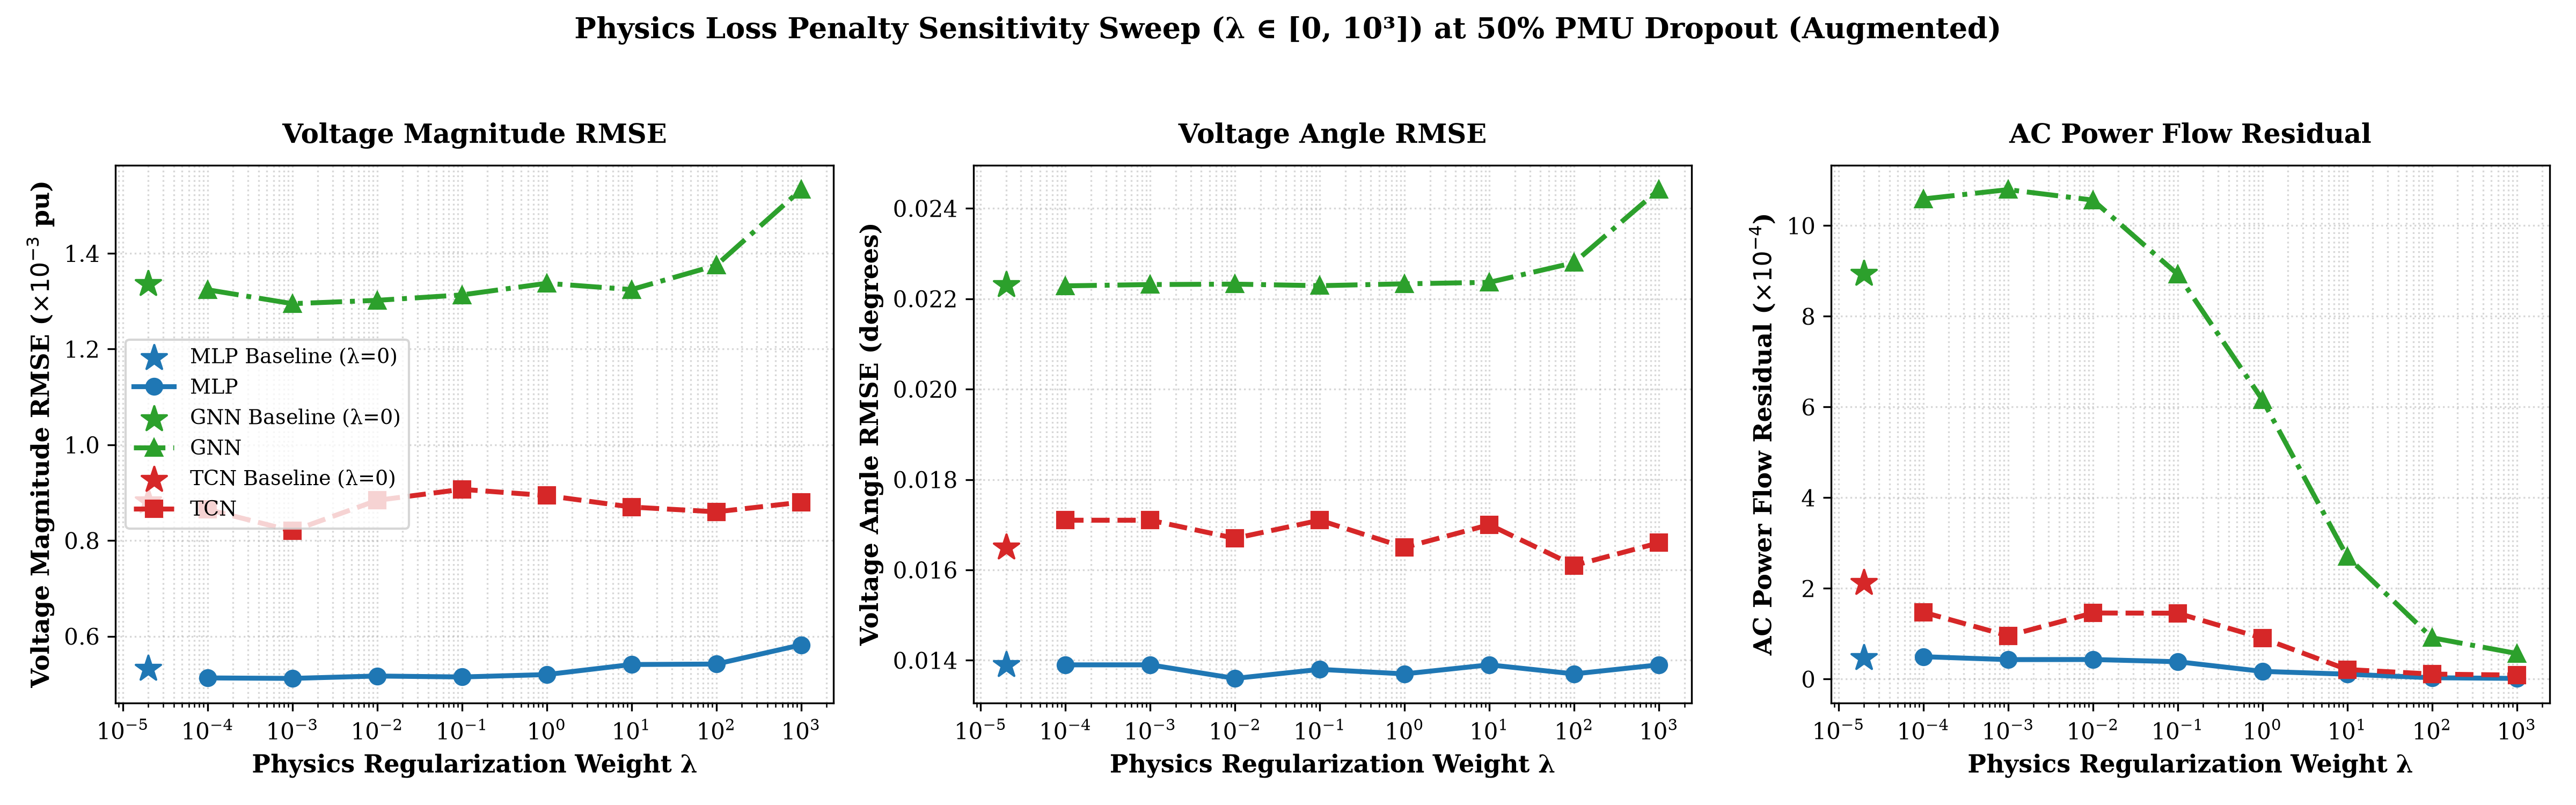
\includegraphics[width=\columnwidth]{lambda_sensitivity_cross_model.png}
    \caption{Physics weight $\lambda$ sensitivity under augmented training at 50\% PMU dropout. Moderate values ($\lambda \le 0.1$) maintain accuracy, while aggressive values ($\lambda \ge 10$) degrade performance---the ``Pareto cliff'' caused by ${\pm}10\%$ pseudo-measurement noise.}
    \label{fig:lambda}
\end{figure}

\subsection{Inference Latency}

Table~\ref{tab:latency} summarizes the CUDA inference latency. The MLP achieves sub-millisecond latency ($0.223$~ms), making it suitable for sub-cycle protection applications running at 50/60~Hz. The GNN and TCN are slower ($1.157$~ms and $2.199$~ms respectively) due to graph convolution and temporal window processing, but both fall well within the 20--50~ms reporting intervals of typical PMU/SCADA systems.

\begin{table}[t]
\centering
\caption{CUDA Inference Latency}
\label{tab:latency}
\footnotesize
\begin{tabular}{lccc}
\toprule
 & \textbf{MLP} & \textbf{GNN} & \textbf{TCN} \\
\midrule
Latency (ms) & 0.223 & 1.157 & 2.199 \\
Relative to MLP & $1.0\times$ & $5.2\times$ & $9.9\times$ \\
\bottomrule
\end{tabular}
\end{table}

% ============================================================
% VI. CONCLUSION
% ============================================================
\section{Conclusion}

This study benchmarked three physics-informed deep learning architectures for distribution system state estimation under progressive sensor dropout. Three consistent trends emerged from the experimental results:

\begin{enumerate}
    \item \textbf{Accuracy vs.\ Resilience:} The MLP provides the highest static accuracy when trained with dropout augmentation ($|V|$~RMSE~$= 0.000515$~pu at 50\% dropout) and the fastest inference ($0.223$~ms). However, without prior exposure to sensor failures, it is the most fragile ($+164\%$ error increase). The TCN provides the strongest resilience against unexpected blackouts ($+25.7\%$ increase) due to its 12-hour temporal receptive field.

    \item \textbf{Topological Horizon:} The 3-layer GNN cannot propagate information across the 17-hop radial feeder. This structural limitation results in accuracy ($0.001295$~pu) that consistently trails both the MLP and TCN, confirming that shallow message-passing networks face a fundamental receptive-field bottleneck on long distribution feeders.

    \item \textbf{Physics Pareto Cliff:} Moderate physics regularization ($\lambda \in [0.001, 0.1]$) is an effective guardrail, but over-penalization ($\lambda \ge 10$) forces models to fit ${\pm}10\%$ pseudo-measurement noise, degrading accuracy sharply.
\end{enumerate}

For deployment, we recommend: (a)~dropout-augmented MLPs for sub-millisecond static estimation where failure patterns can be anticipated during training; (b)~TCNs for mission-critical resilience against unmodeled communication blackouts; and (c)~physics regularization calibrated against pseudo-measurement quality, keeping $\lambda \le 0.1$ under typical ${\pm}10\%$ forecast noise.

% ============================================================
% REFERENCES
% ============================================================
\begin{thebibliography}{10}

\bibitem{schweppe1970}
F.~C. Schweppe and J.~Wildes, ``Power system static-state estimation, Part~I: Exact model,'' \textit{IEEE Trans. Power Apparatus and Systems}, vol.~PAS-89, no.~1, pp.~120--125, Jan. 1970.

\bibitem{primadianto2017}
A.~Primadianto and C.-N. Lu, ``A review on distribution system state estimation,'' \textit{IEEE Trans. Power Systems}, vol.~32, no.~5, pp.~3875--3883, Sep. 2017.

\bibitem{mestav2019}
K.~R. Mestav, J.~Luber, R.~Batber, and L.~Tong, ``Bayesian state estimation for unobservable distribution systems via deep learning,'' \textit{IEEE Trans. Power Systems}, vol.~34, no.~6, pp.~4910--4920, Nov. 2019.

\bibitem{iliadis2025}
N.~A. Iliadis, S.~Moffat, and B.~C. Pal, ``Physics-informed neural network for distribution system state estimation,'' \textit{IEEE Trans. Power Systems}, 2025, early access.

\bibitem{raghuvamsi2024}
B.~Raghuvamsi, V.~K. Teeparthi, and D.~M. V. Kumar, ``Physics-informed temporal convolutional autoencoder for distribution system state estimation,'' \textit{Electric Power Systems Research}, vol.~232, 2024, Art. no.~110350.

\bibitem{ngo2024}
D.~T. Ngo, C.~D. Nguyen, and S.~R. Lee, ``Hybrid graph neural network and Kalman filter for distribution system state estimation,'' \textit{IEEE Access}, vol.~12, pp.~45232--45244, 2024.

\bibitem{hu2025}
J.~Hu, Z.~Ye, Y.~Tang, and H.~Sun, ``Physics-embedded graph attention network for distribution system state estimation,'' \textit{IEEE Trans. Smart Grid}, 2025, early access.

\bibitem{baran1989}
M.~E. Baran and F.~F. Wu, ``Network reconfiguration in distribution systems for loss reduction and load balancing,'' \textit{IEEE Trans. Power Delivery}, vol.~4, no.~2, pp.~1401--1407, Apr. 1989.

\bibitem{kipf2017}
T.~N. Kipf and M.~Welling, ``Semi-supervised classification with graph convolutional networks,'' in \textit{Proc. Int. Conf. Learning Representations (ICLR)}, 2017.

\bibitem{bai2018}
S.~Bai, J.~Z. Kolter, and V.~Koltun, ``An empirical evaluation of generic convolutional and recurrent networks for sequence modeling,'' \textit{arXiv:1803.01271}, 2018.

\end{thebibliography}

\end{document}
